\subsection{Considerações sobre o Logisim Evolution}

Haja vista a importância desses elementos de memória, o Logisim Evolution possui implementações prontas em circúitos integrados, as quais serão utilizadas a partir deste ponto no documento:

\begin{figure}[H]
    \centering
    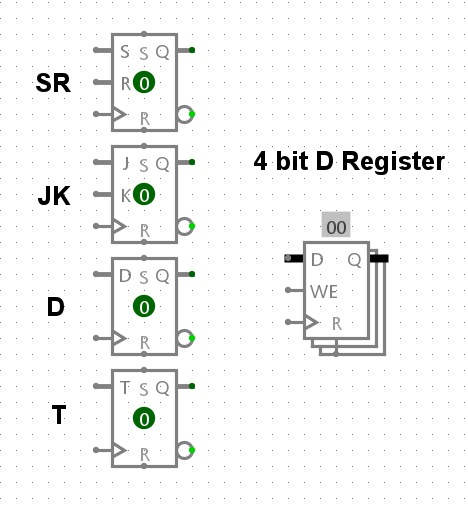
\includegraphics[width=0.5\linewidth]{images/memory-cis.png}
    \caption{Elementos de memória no Logisim Evolution}
    \label{fig:FF-logisim}
\end{figure}

Note que nesses flip flops exitem duas entradas e uma saída extras respectivamente $S, R$ e $\lnot Q$ (saída abaixo de $Q$ com circulo representando NOT).

\begin{itemize}
    \item $S_t = 1 \rightarrow Q_t = 1$, mesmo que sem pulso de clock 
    \item $R_t = 1 \rightarrow Q_t = 0$, mesmo que sem pulso de clock
    \item $S_t = R_t = 1 \rightarrow Q_t = 0$ 
\end{itemize}

Além disso, a entrada do clock é representada por: 

\begin{figure}[H]
    \centering
    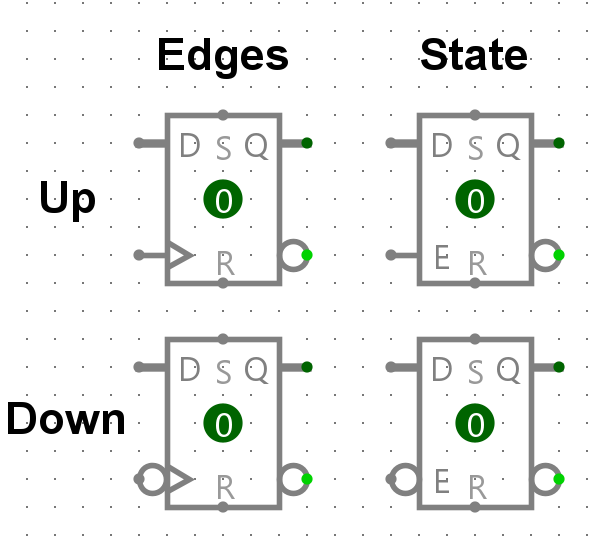
\includegraphics[width=0.4\linewidth]{images/clk-in-logisim.png}
    \caption{Representações de entrada de clock no Logisim Evolution}
    \label{fig:clk-in-logisim}
\end{figure}
